\documentclass[a4paper,11pt]{article}
%\usepackage[T1]{fontenc}
\usepackage[utf8]{inputenc}
%\usepackage{lmodern}
\usepackage[french]{babel}
\usepackage{amsmath} % math
\usepackage{amsfonts}% math
\usepackage{amssymb} % math
% \usepackage{gensymb} % math
\usepackage{graphicx} % images
\usepackage{float}    % images float
% \usepackage{qtree}    % dessiner des arbres %% => texlive-humanities
\usepackage{url}
	\urlstyle{sf}
\usepackage[usenames]{color}
\usepackage[french]{varioref} % \vref and \vpageref
\usepackage[top=2.5cm, bottom=2.5cm, left=2.5cm, right=2.5cm]{geometry}
\usepackage[backgroundcolor=yellow]{todonotes} %% todonotes: \listoftodos & \todo{Some note or other.} & \missingfigure{}


\definecolor{codeBlue}{rgb}{0,0,1}
\definecolor{webred}{rgb}{0.5,0,0}
\definecolor{codeGreen}{rgb}{0,0.5,0}
\definecolor{codeGrey}{rgb}{0.6,0.6,0.6}
\definecolor{webdarkblue}{rgb}{0,0,0.4}
\definecolor{webgreen}{rgb}{0,0.3,0}
\definecolor{webblue}{rgb}{0,0,0.8}
\definecolor{orange}{rgb}{0.7,0.1,0.1}

\usepackage{caption}
\renewcommand{\familydefault}{\sfdefault}
\usepackage{listings}		% Pour l'insersion de fichiers de codes sources.
\lstset{
	  language=SQL,
	  frame=single,
	  flexiblecolumns=true,
	  numbers=none, % left
	  stepnumber=1,
	  numberstyle=\ttfamily\tiny,
	  keywordstyle=\ttfamily\textcolor{blue},
	  stringstyle=\ttfamily\textcolor{red},
	  commentstyle=\ttfamily\textcolor{green},
	  breaklines=true,
	  extendedchars=true,
	  basicstyle=\ttfamily\scriptsize,
	  showstringspaces=false
	}

\IfFileExists{fourier.sty}{\usepackage{fourier}}{\typeout{! WARNING: Fourier package not included: skip it}}

%%%%%%%%%%%%%%%%%%%%

\newcommand{\userstory}[3]{En tant #1, je voudrais \textbf{#2}, ainsi \textbf{#3}.\\}
\newcommand{\etauto}[2]{\userstory{qu'\textit{automobiliste}}{#1}{#2}}
\newcommand{\etgp}[2]{\userstory{que \textit{gestionnaire de parking}}{#1}{#2}}

%%%%%%%%%%%%%%%%%%%%

\title{\texttt{LINGI2172}: Database\\Mission 3 \& 4}
\author{Matthieu \textsc{Baerts} \and Benoît \textsc{Baufays} \and Julien \textsc{Colmonts} \and Alex \textsc{Vermeylen}}
\date{\today}

\begin{document}


\maketitle
\tableofcontents

%%%%%%%%%%%%%%%%%%%%
\section*{Introduction}
Ce document décrit en détails notre application de gestion de parkings: \textit{Parking App}. Une description accompagnée des buts et besoins du programme ainsi que les différentes histoires utilisateurs possibles y sont présentés ci-dessous.

À cela s'ajoute également les explications de notre application Android, la méthode de programmation utilisée et les scripts de notre base de données.


\section{Vision document}

Construire une application de réservation et de gestion de parkings permet :
\begin{itemize}
  \item Pour un automobiliste :
  \begin{itemize}
  	\item Trouver une place de parking la plus proche ou la moins cher
    \item Gérer ses abonnements de parking
    % Source: https://play.google.com/store/apps/details?id=net.osmand.parkingPlugin
    \item Retrouver un emplacement de parking
    \item Être averti lorsque le temps de parking est dépassé.
  \end{itemize}
  \item Pour un gestionnaire de parking :
  \begin{itemize}
    \item Gérer les abonnements de son parking
    \item Avoir des statistiques détaillées d'utilisation de son parking
  \end{itemize}
\end{itemize}


\section{Description}

La Parking App est une application permettant de trouver les places de parking libres les plus proches ou de comparer les différentes offres.  L'application se basera sur une base de données contenant les parkings avec le nombre de places totales, la grille de tarif ainsi que leur localisation et, éventuellement, des informations complémentaires comme le nombre de places de parkings handicapés ou la présence d'un défibrillateur.\\

Afin de garder les informations de parking à jour, le gestionnaire de parkings peut modifier les informations relatives à son ou ses parkings.  Avec l'historique de fréquentation et le temps d'occupation de chaque parking, le gestionnaire de parkings pourra avoir des statistiques détaillées sur son parking.  Pour l'utilisateur, il pourra savoir s'il est déjà venu dans le parking et, éventuellement, voir ses évaluations.



\section{Goals \& software requirements}\label{goals}

\begin{itemize}
  \item Toute voiture qui entre dans un parking finira tôt ou tard par en sortir.
  \item Une voiture alimentée par un carburant interdit dans un certain parking ne pourra jamais se garer dans ce parking.
  \item Un véhicule dont la hauteur dépasse la hauteur maximale d'un parking ne pourra jamais se garer dans ce parking.
  \item Un utilisateur voulant se garer en dehors des horaires d'ouverture d'un parking spécifique ne pourra jamais effectuer cette action à cet horaire précis.
  \item Un utilisateur qui sort d'un parking finira tôt ou tard par donner son feedback.
  \item Un parking sera toujours ouvert au moins pendant une période pendant la semaine.
  \item Un parking acceptera au moins un type de carburant.
\end{itemize}

\section{User Stories}\label{users-stories}
\subsection{Pour l'automobiliste}
  \noindent
  \etauto{obtenir la liste des parkings aux alentours}{je pourrai choisir quel parking m'intéresse}
  \etauto{obtenir la liste des parkings près d'un endroit}{je pourrai planifier l'endroit où je compte me garer}
  \etauto{classer la liste avec les parkings les plus proches}{je pourrai me garer tout près}
  \etauto{classer la liste en commençant par les parkings les moins chers}{je pourrai faire des économies}
  \etauto{filtrer la liste avec uniquement les parkings disposant d'au-moins une place libre}{je pourrai me garer avec la certitude d'avoir une place}
  \etauto{filtrer la liste avec uniquement les parkings disposant d'un défibrillateur}{je pourrai être rassuré en cas de problème}
  \etauto{filtrer la liste avec uniquement les parkings disposant de place réservées aux handicapés}{je pourrai trouver une place plus large et près de la sortie} % je pourrais emmener papy/la Charlie team/autre?
  \etauto{filtrer la liste avec uniquement les parkings acceptant mon abonnement}{je pourrai m'y garer avec ma carte}
  \etauto{retrouver un parking avec son nom ou identifiant}{je pourrai retrouver un parking}
  \etauto{avoir toutes les informations d'un parking dans la liste}{je pourrai me faire une idée sur le parking en question}
  \etauto{mettre un parking en favori}{je pourrai rapidement retrouver un parking}
  \etauto{indiquer un rappel lié à un parking}{je pourrai rejoindre le parking avant le délai maximum}
  \etauto{gérer mes abonnements de parking}{je pourrai consulter mon compte et mes informations liés à ces abonnements}
  \etauto{avoir un historique des recherches}{je pourrai rapidement retrouver une précédente recherche}
  \etauto{avoir un historique des parkings visités}{je pourrai retrouver les parkings précédemment visités}
  \etauto{indiquer une note/commentaire pour un parking}{je pourrai informer les autres utilisateurs}
  % DOUBLON ! \etauto{marquer certains parkings en favoris}{je pourrais facilement les retrouver}
%  \etauto{}{}
  %\etauto{danser nu avec des fougères}{je gagnerai un pari}

\subsection{Pour le gestionnaire de parking}
  \noindent
  \userstory{que \textit{futur gestionnaire de parking}}{pouvoir me créer un compte spécial gestionnaire de parking}{gérer mes parkings}
  \etgp{pouvoir rajouter mon parking (avec toutes ses données associées) dans l'application}{il sera visible pour les utilisateurs}
  \etgp{pouvoir modifier les données que j'ai précédemment entrées pour un de mes parkings}{chaque information pourra être à jour}
  \etgp{pouvoir supprimer ou fermer un de mes parkings}{un parking ne sera plus présent/visible dans l'application} 
  \etgp{pouvoir consulter la liste des abonnés à un de mes/tous mes parkings}{je pourrai faire des statistiques}
  \etgp{pouvoir consulter le nombre d'automobilistes présents à un de mes/tous mes parkings}{je pourrai faire des statistiques}
  \etgp{pouvoir consulter divers données statistiques}{je pourrai mieux adapter l'infrastructure du parking}
%  \etgp{}{}

\section{ER Schema}
\begin{figure}[H]
	\begin{center}
		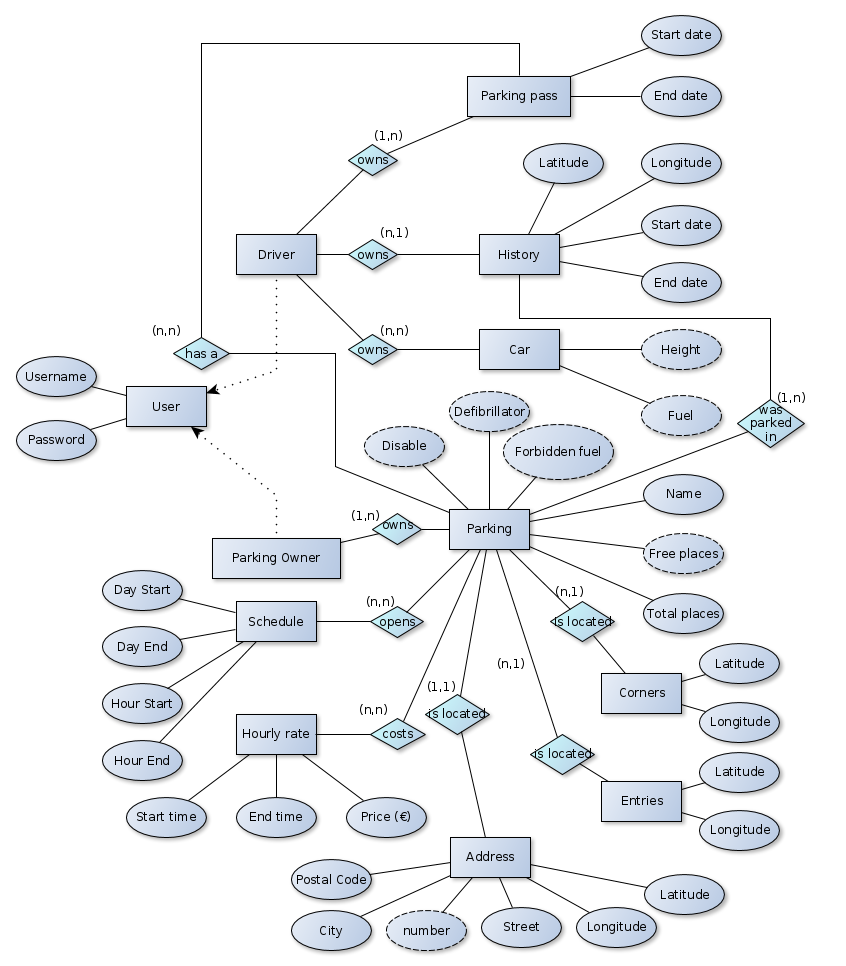
\includegraphics[width=\textwidth]{schema_db_er.png}
		\caption{ER Schema}
		\label{fig:er}
	\end{center}
\end{figure}
Sur la figure \vref{fig:er}, comme l'entité \emph{Driver} et \emph{Parking Owner} ont des attributs en commun (\emph{Username} et \emph{Password}) mais qu'ils n'ont pas le même rôle (trouver une place de parking et s'occuper d'un parking respectivement), nous avons décidé de créer une entité \emph{User}.\\
Il est aisé de lier ce schéma à nos Users Stories. Par exemple, la User Story "\textit{En tant qu’automobiliste, je voudrais avoir un historique des parkings visités, ainsi je pourrai retrouver les parkings précédemment visités}" est satisfaite via le lien existant entre l'entité \emph{Driver} et l'entité \emph{History}.

\section{Logical Schema}
Nous listons les \textit{relvars} ci-dessous en anglais pour être en harmonie avec le nom des variables.
%\begin{otherlanguage}{english}
\begin{itemize}
  \item User \texttt{USERID} has \texttt{USERNAME} name, can connect with \texttt{PASSWORD} password and is from type \texttt{TYPE}.
  \item Parking pass \texttt{PASSID} starts at \texttt{START} date, ends at \texttt{END} date and belongs to \texttt{USER} user.
  \item Parking \texttt{PARKINGID} has \texttt{NAME} name, has/hasn't a \texttt{DEFIBRILATOR} defibrillator and a \texttt{DISABLE} place for disabled people, counts \texttt{FREESPACE} free parking slots under a total of \texttt{TOTALSPACE} parking slots, accepts vehicules of \texttt{HEIGHT} height.
  \item Parking pass \texttt{PASS} is related to \texttt{PARKING} parking
  \item Parking \texttt{PARKING} doesn't accept \texttt{FORBIDDENFUEL} fuel
  \item Parking \texttt{PARKING} opens from \texttt{DAYSTART} to \texttt{DAYEND}, at \texttt{HOURSTART} to \texttt{HOUREND}.
  \item Parking \texttt{PARKING} is located at address \texttt{STREET NUMER}, \texttt{ZIPCODE}, \texttt{CITY}, \texttt{COUNTRY}, and precisely at \texttt{LATITUDE}, \texttt{LONGITUDE} coordinates
  \item Car \texttt{CARID} belongs to \texttt{USER} user, is located at \texttt{LATITUDE}, \texttt{LONGITUDE} coordinates, uses \texttt{FUEL} fuel and measures \texttt{HEIGHT} height
  \item Parking entrance of \texttt{PARKING} parking is located at \texttt{LATITUDE}, \texttt{LONGITUDE} coordinates
  \item Parking corners from parking \texttt{PARKING} is located at \texttt{LATITUDE}, \texttt{LONGITUDE} coordinates
  \item Parking entrance from parking \texttt{PARKING} is located at \texttt{LATITUDE}, \texttt{LONGITUDE} coordinates
  \item Fuel \texttt{FUELID} refers to \texttt{NAME} fuel
  \item History remembers a \texttt{CAR} car parked in \texttt{PARKING} parking between \texttt{START} and \texttt{END} dates
\end{itemize}
%\end{otherlanguage}

\begin{figure}[H]
	\begin{center}
		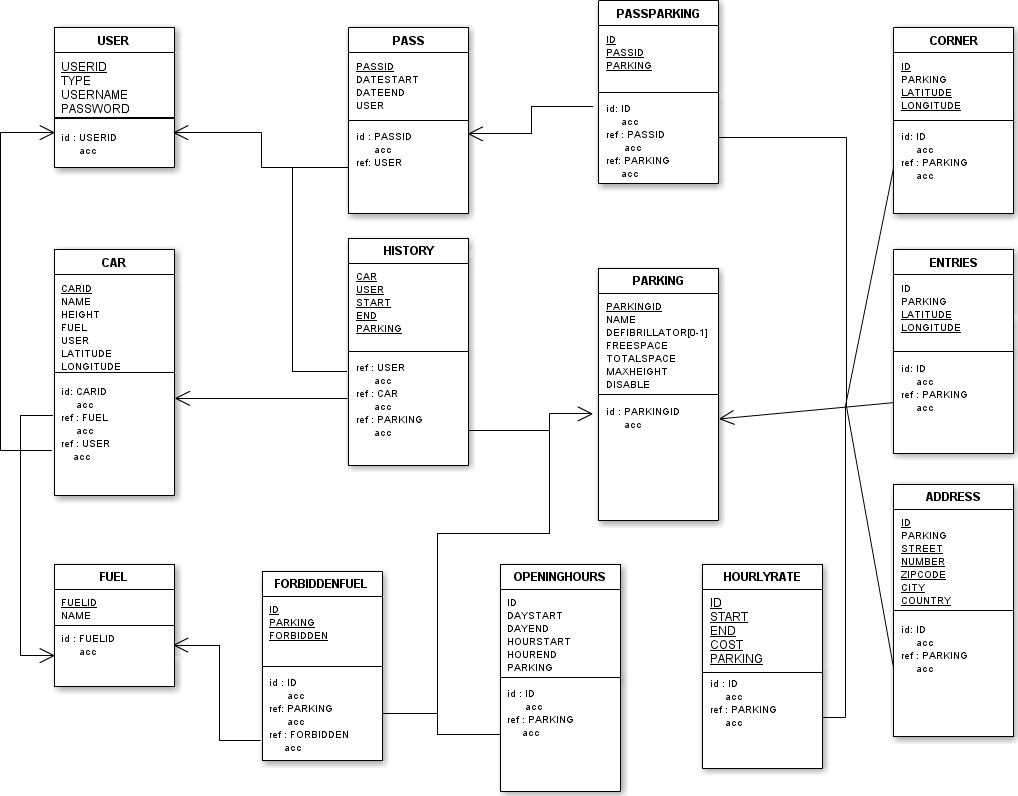
\includegraphics[width=1\textwidth]{schema_logic_new-M4.png}
		\caption{Logical Schema (le fichier original est joint à ce rapport)\\Les champs soulignés représentent des champs uniques.}
		\label{fig:logic}
	\end{center}
\end{figure}

Nous avons inclu les contraintes suivantes sur les objets:
\begin{itemize}
	\item Carburant : certains types de carburant, comme le \emph{LPG}, ne sont pas autorisés dans tous les parkings.  Afin d'avertir l'utilisateur que son véhicule sera refusé dans un parking n'autorisant pas son carburant, nous avons ajouté une contrainte de carburant.  Elle se situe entre le véhicule de l'utilisateur et le parking désiré. La base de données ne pourra donc pas contenir dans sa table \textit{History} un lien entre un véhicule et un parking qui ne respecte pas les interdictions liées à ce parking.
    \item Hauteur : chaque parking a une hauteur maximale et chaque véhicule a une hauteur.  Afin d'informer l'utilisateur sur la possibilité de faire rentrer son véhicule dans le parking désiré, nous avons ajouté une contrainte visant à limiter la visibilité de l'utilisateur sur les parkings ayant une hauteur maximale inférieure à la hauteur de leur véhicule;
    \item Ouverture : chaque parking a des heures d'ouvertures.  Afin de proposer uniquement les parkings ouverts, nous avons ajouté une contrainte entre l'historique (qui contient également l'occupation courante d'un parking) et les horaires du parkings.  De plus, afin de garder l'intégrité de la base de données, chaque entrée de l'historique devra satisfaire cette contrainte, en ce compris pour la date de sortie.  Cette contrainte supplémentaire nous permettra d'indiquer à l'utilisateur les plages horaires durant lesquels il pourra récupérer son véhicule.
    \item Places restantes : chaque parking a une capacité maximale et comme on désire ne proposer que les parkings disposant encore d'au-moins une place libre, nous devons nous assurer que le nombre de places libres ne dépasse pas le nombre de places total dans ce parking.  Cette contrainte nous permet de préserver l'intégrité de la base de données, même après une modification incorrecte ou un problème lié au software.  Cette contrainte se situe uniquement dans la table \textit{Parking}.
    \item Jour d'ouverture : comme nous avons une contrainte (\emph{Ouverture}) qui nous permet de proposer uniquement les parkings ouverts, nous devons nous assurer que les informations reprises dans la table couvrant les horaires d'ouvertures sont correctes.  Ainsi, nous avons ajouté la contrainte que le jour de début et de fin doit bien correspondre à un jour de la semaine.  Par facilité pour vérifier cette contrainte, nous avons encodé cette donnée en \textit{Integer}.  Le champ ne doit donc contenir que des chiffres allant de 0 à 6 compris.
\end{itemize}

Outre toutes ces contraintes, nous avons également une contrainte que chaque type dans la base de données doit être correct.  Ainsi, pour les heures d'ouvertures ou les dates, nous avons ajouté, comme contrainte implicite, que les informations contenues dans la base de données reflètent bien les données désirées (\textit{Time}, \textit{DateTime}).

\section{Scripts en SQL et Tutorial D}
Les scripts pour créer les bases de données en SQL et Tutorial D sont joints à ce document et disponibles en annexe \vref{sql} pour SQL et en annexe \vref{tutoriald} pour Tutorial D.\\
Concernant la base de données en SQL, nous allons utiliser SQLite pour des raisons pratiques puisque nous avons réalisé une application mobile où l'intégration avec SQLite est gérée nativement. Il est donc important de noter qu'il existe certainement différences avec PostgreSQL, notamment que des types \texttt{INT} pouvant être \texttt{NULL}.

\section{Organisation dans l'application Android}
Chaque objet du schéma de la base de données a été transformé en classe Java et implémentant l'interface \emph{Model}, interface qui reprend les méthodes génériques spécifiques à un objet d'une base de données.\\
Nous avons également ajouté des objets "\textit{bases de donnée}s" pour chaque \emph{Model} afin d'effectuer tous les liens entre notre application et notre base de données. Enfin, nous avons préféré séparer la gestion de la base de données entre tous les \emph{Model} afin de minimiser les locks d'ouvertures sur la base de données ainsi que pour offrir un système schématique pour l'ajout d'un nouvel objet via une classe abstraite. Ce explique également le nombre important de classes dans le package \texttt{com.charlyparkingapps.db}.

\section{Filtre}
La partie filtre est le c\oe ur de notre application puisqu'elle permet d'effectuer des requêtes à travers plusieurs tables et de faire intervenir plusieurs contraintes comme le carburant ou la hauteur.\\
Comme la fonction filtre doit renvoyer une liste de \textit{Parking}'s, nous avons d'abord pensé à une seule requête que nous construirions en fonction des filtres choisis.  Ce système permet l'exécution d'une seule requête personnalisée et traitant uniquement les filtres désirés.\\
Voici un exemple:
\begin{lstlisting}[language=Java]
String totPlaces = prefs.getInt(FiltersActivity.TOTALPLACES_PREF, 0)!=0 ? "AND totalPlaces >= "
				+ prefs.getInt(FiltersActivity.TOTALPLACES_PREF, 0) + " " : "";
Cursor cursor = myBDD.rawQuery(
		"SELECT * FROM Parking P, ForbiddenFuel FF, Fuel F "
        + "WHERE (P.parkingId = FF.parking OR P.parkingId != FF.parking) "
        + "AND defibrillator IN (" + def + ") "
        + "AND disable IN (" + dis + ") "
		+ getFuels + totPlaces + freePlaces + oneFree + cos, null);
\end{lstlisting}

Ainsi, comme on peut le voir dans cet exemple, nous n'ajoutons une condition (\texttt{AND ...}) que lorsque le test nous informe que la "\textit{préférence}" (le filtre) est présente et que la méthode utilisée pour en récupéré la valeur ne renvoie pas la valeur par défaut.  Nous aurions pu réaliser une requête plus simple incluant tous les filtres avec les paramètres par défauts pour les dits filtres non utilisés, mais nous aurions alors eu une requête plus longue et lourde et donc, plus lente pour le même résultat.\\

Comme il s'agissait de retrouver un ensemble de \textit{Parking}'s, nous avons préféré ensuite nous tourner vers une fonction en \emph{SQL} nous retournant une table de Parking.  Nous aurions pu passer par une \emph{View} mais nous n'avons pas trouvé de moyen élégant de passer les filtres en paramètres.  Nous aurions pu également utiliser un \emph{Trigger} qui mettrait à jour la table des parkings dès qu'un nouvel objet \textit{Parking} serait ajouté ou modifié mais, \emph{Android} imposant d'utiliser \emph{SQLite}, qui ne permet pas les conditions dans les \emph{Triggers}, de tels \emph{Triggers} étaient impossibles à implémenter.  De plus, les fonctions n'étant pas non plus gérées par \emph{SQLite}, nous n'en avons pas utilisées et nous donnons ici le code tel que nous l'avons prévu à titre explicatif.
\begin{lstlisting}[language=SQL]
CREATE FUNCTION getParkings (@def TEXT, @dis TEXT, @fuels TEXT, @totalP INT, @freeP INT, @price INT)
RETURNS TABLE
AS
RETURN
  SELECT * FROM Parking P, ForbiddenFuel FF, Fuel F
  WHERE (P.parkingId = FF.parking OR P.parkingId != FF.parking)
    AND defibrillator IN (@def) 
    AND disable IN (@dis)
    AND (P.parkingId = FF.parking)
    AND F.name NOT IN (@fuels) ND totalPlaces >= @totalP 
    AND freePlaces >= @freeP
    AND freePlaces > 0
    AND P.ParkingId IN (SELECT parking FROM HourlyRate WHERE cost <= @price)
\end{lstlisting}


\section{Importation de données}
Afin de peupler notre base de données, nous sommes parti du gestionnaire de parking européen \emph{Vinci Park}\footnote{Vinci Park est une filiale de Vinci Concessions chargée de l'exploitation de parkings dans le monde.\\(\url{http://www.vincipark.com})} qui permet, depuis son site, de trouver le parking le plus proche d'une adresse.  Comme il s'agit d'une simple requête \emph{GET}, nous avons effectué plusieurs recherches avec \emph{Nice}, \emph{Paris}, \emph{Monaco} et \emph{Bruxelles}.\\

Avec la liste de résultats, nous avions accès à la fiche de chaque parking contenant son adresse postale, son horaire, ses tarifs et ses services.  Hélas, nous n'avions pas les coordonnées géographiques de parkings sur le site.  Nous avons alors utilisé un outils en ligne\footnote{\url{http://www.gps-coordinates.net}} permettant de convertir une adresse en coordonnées GPS.\\

Si vous visitez le site, vous verrez que \emph{Vinci Park} a une politique globale concernant la tarification, ce qui rend les tests du filtre beaucoup moins intéressant.  Pour cette raison, nous nous sommes permis de modifier la grille tarifaire affichée par \emph{Vinci Park} ainsi que la hauteur maximale autorisée.


\section{Des \textit{Users Stories} à la base de données}
Suite à notre discussion avec le Professeur Lambeau, nous nous permettons d'ajouter une section expliquant le cheminement que nous avons suivi pour générer le schéma de la base de données à partir des \textit{Users Stories}.\\

En effet, avant l'apparition de la méthode \emph{Agile}, presque tous les projets suivaient le modèle \emph{Waterfall} (ou assimilé avec le V model) dans lequel la base de données, et donc son schéma, était totalement défini avant la phase de production.  Ce système avait l'avantage d'avoir une vue globale du système relationnel mais sa définition obligeait de travailler d'une manière totalement théorique et sur les concepts voulus pour l'application.\\

En utilisant la méthode \emph{Agile}, on a voulu se libérer de la rigidité imposée par la phase de réflexion précédent la phase  de production.  Pour y arriver, on défini d'abord un ensemble d'\emph{Users Stories}, rassemblant les différentes actions qui rassemblent l'ensemble des \emph{features} de l'application. Ainsi, en travaillant de \emph{Feature} en \emph{Feature}, nous arrivons à l'application finale.\\

Pour ce projet, nous sommes parti de la définition d'\emph{Users Stories} qui définissent l'ensemble des \emph{Features} désirées pour notre application.  Avant de développer l'application, nous avons classé les différentes \emph{Users Stories} en catégories, comme présenté dans la section \vref{users-stories}. 
Ce regroupement par catégorie nous permet de définir un domaine consistant pour un ensemble de \emph{User Stories} manipulant un set d'objets communs.\\
En partant de ces catégories, nous avons dérivés les différents objets interagissants ensemble ainsi que leurs informations échangées. Ainsi, pour définir les différents objets, nous sommes partis principalement de l'assertion \emph{En Tant que} qui défini le domaine de l'\emph{User Story} suivi de l'assertion \emph{je voudrais} qui indique l'action et l'objet sur lequel il est executé.\\
Grâce à ces deux assertions, nous avons pu migrer notre schéma de base de données afin d'y ajouter les objets permettant d'appliquer l'\emph{User Story} sur notre application. Si l'objet existait déjà dans la base de données et avait été créé dans une catégorie d'\emph{Users Stories} différente, nous pouvons en dériver, généralement, une relation ternaire contenant des informations supplémentaires.\\
L'ajout d'un nouveau champ à un objet se fait seulement après avoir vérifié qu'aucune requête sur le schéma ne peut fournir l'information désirée.\\
En analysant l'assertion \emph{ainsi}, nous pouvons également dériver des relations impliquant plus que deux tables, comme des relations \textit{un à plusieurs} ou \textit{plusieurs à plusieurs}.\\
Enfin, pour ajouter les contraintes, nous sommes parti de la section \vref{goals} \textit{Goals \& software requirements}, et ce, après avoir parcouru l'ensemble des \emph{Users Stories}.  Cette action, en deux temps, nous permet d'être certains d'avoir toutes les contraintes voulues dans les \textit{requirements} et ce, sur tous les objets constituant notre schéma.\\

Ainsi, en suivant cette procédure, basée sur notre petite expérience de la méthode \textit{Agile}, nous avons pu générer un schéma de base de données se rapprochant le plus possible d'un schéma généré via le modèle \emph{Waterfall} (ou assimilé) tout en gardant la modularité de la méthodologie \emph{Agile}.\\

À noter également que certains frameworks que nous avons déjà utilisés sont peut-être plus adaptés à cette méthode \textit{Agile}. Par exemple, il y a le framework \textit{Ruby On Rails} qui permet de facilement faire des mises à jour de la structure de la base de données et ajouter facilement de nouveaux liens entre objets par après.



\section{Utilisation de l'application en elle-même}
Le binaire \texttt{.apk} est joint à ce document pour faciliter les éventuels tests.

\subsection{Sources}
Le code source est également joint et il peut être importé facilement avec l'outil d'import d'Eclipse. À noter également que comme seule dépendance, il faut ajouter la lib \texttt{google-play-services\_lib}:
\begin{itemize}
	\item Pour cela, il faut tout d'abord installer les Google Play Services: dans Eclipse, se rendre dans le menu \textit{Window} / \textit{Android SDK Manager} / cocher et installer les Google Play Services.
    \item Importer la bibliothèque dans le workspace en utilisant l'outil d'import d'Eclipse pour un projet Android et indiquer le chemin de la lib, par exemple: \texttt{VOTRE\_ANDROID\_SDK/extras/goo\-gle/google\_play\_services/libproject/google-play-services\_lib}.
    \item Dans les propriétés du projet \textit{CharlyParkingApp}, ajouter \texttt{google-play-services\_lib} comme bibliothèque utilisée.
\end{itemize}

\subsection{Application}
En lançant l'application pour la première fois, les identifiants de l'utilisateur sont demandés. L'utilisateur principal pour les tests se prénome \textit{user} avec le mot de passe \textit{abcd}.\\

Ensuite, tous les parkings sont affichés sur la carte (n'ayant pas trop de parkings dans la base de données, ceci ne pose pas de problème). Au-dessus à gauche se trouve le menu principal pour permettre d'afficher les différentes catégories du programme: les filtres, le profile, les voitures, l'historique et les parkings. Sur certaines vues comme celle liées aux voiture (\textit{My cars}), on retrouve également d'autres fonctionnalités dans le menu supérieur droit et montre très bien les liens existants entre une voiture, l'endroit où elle a été garée la dernière fois, le parking pour le moment utilisé, toutes les voitures garées pour le moment, etc. Depuis cette vue, il est également possible de modifier les voitures et en ajouter.\\

À noter également que certaines vues et fonctionnalités pas tellement liées à la gestion de la base de données sont parfois dans un état très "brut".


\section*{Conclusion}
Grâce aux différentes descriptions énoncées, nous avons une meilleure vue d'ensemble du programme et ceci devrait donc permettre à quiconque de s'imaginer comment l'application va fonctionner et à quels buts elle va servir.

\newpage
\appendix

\section{Script SQL}\label{sql}
\begin{lstlisting}
DROP TABLE IF EXISTS "Address";
DROP TABLE IF EXISTS "Car";
DROP TABLE IF EXISTS "Corners";
DROP TABLE IF EXISTS "Entries";
DROP TABLE IF EXISTS "ForbiddenFuel";
DROP TABLE IF EXISTS "Fuel";
DROP TABLE IF EXISTS "History";
DROP TABLE IF EXISTS "HourlyRate";
DROP TABLE IF EXISTS "OpeningHours";
DROP TABLE IF EXISTS "Parking";
DROP TABLE IF EXISTS "User";


CREATE TABLE Address(addressId INTEGER NOT NULL PRIMARY KEY AUTOINCREMENT, 
	parking INTEGER NOT NULL, 
	street TEXT NOT NULL, 
	number INTEGER NOT NULL, 
	city TEXT NOT NULL, 
	zip INTEGER NOT NULL, 
	country TEXT NOT NULL, 
	latitude DOUBLE NOT NULL, 
	longitude DOUBLE NOT NULL, 
	FOREIGN KEY(parking) REFERENCES Parking(parkingId));
INSERT INTO "Address" VALUES(0, 1, 'Place Sainte Barbe', 1, 'Louvain-la-Neuve', 1348, 'BE', 50.667408, 4.62202);
INSERT INTO "Address" VALUES(1, 3, 'Place de Hotel de Ville', 0, 'Saint-Quentin', 2100, 'FR', 49.846122, 3.287457);
INSERT INTO "Address" VALUES(2, 4, 'Cours Saleya', 0, '6300', 'Nice', 'FR', 43.695607, 7.49227);
INSERT INTO "Address" VALUES(3, 5, 'Place du XVe Corps', 0, 'Nice', 6000, 'FR', 43.7072969, 7.2801912);
INSERT INTO "Address" VALUES(4, 6, 'Place du Palais de Justice', 0, 'Nice', 6000, 'FR', 43.696672, 7.273752);
INSERT INTO "Address" VALUES(5, 7, 'Rue de Ponthieu', 59, 'Paris', 75008, 'FR', 48.8721412, 2.3049417);
INSERT INTO "Address" VALUES(6, 8, 'Rue des Fosses', 19, 'Braine-l Alleud', 1420, 'BE', 50.6836196, 4.3712134);
INSERT INTO "Address" VALUES(7, 9, 'Place de la Justice', 16, 'Bruxelles', 1000, 'BE', 50.8439031, 4.3546111);
INSERT INTO "Address" VALUES(8, 10, 'Boulevard Emile Jacqmain', 14, 'Bruxelles', 1000, 'BE', 50.852511, 4.3529971);
INSERT INTO "Address" VALUES(9, 10, 'Boulevard du Jardin Botanique', 29, 'Bruxelles', 1000, 'BE', 50.854461, 4.3601597);
INSERT INTO "Address" VALUES(11, 12, 'Rue du Damier', 26, 'Bruxelles', 1000, 'BE', 50.8532061, 4.3580816);
INSERT INTO "Address" VALUES(12, 13, 'Rue des Cendres', 8, 'Bruxelles', 1000, 'BE', 50.8546555, 4.3598398);
INSERT INTO "Address" VALUES(13, 14, 'Place du Nouveau Marche aux Grains', 1, 'Bruxelles', 1000, 'BE', 50.8507354, 4.3449141);
INSERT INTO "Address" VALUES(14, 15, 'Rue de Flandre', 60, 'Bruxelles', 1000, 'BE', 50.851665, 4.3462069);
INSERT INTO "Address" VALUES(15, 16, 'Place De Brouckere', 1, 'Bruxelles', 1000, 'BE', 50.8510611, 4.3524389);
INSERT INTO "Address" VALUES(16, 17, 'Boulevard de Waterloo', 1, 'Bruxelles', 1000, 'BE', 50.8388739, 4.3613843);
INSERT INTO "Address" VALUES(17, 18, 'Rue de l Ecuyer', 15, 'Bruxelles', 1000, 'BE', 50.8492771, 4.3534652);


CREATE TABLE Car (carId INTEGER PRIMARY KEY AUTOINCREMENT NOT NULL,
	name TEXT NOT NULL,
	height INTEGER DEFAULT 0,
	fuel INTEGER DEFAULT 0,
	user INTEGER NOT NULL,
	latitude DOUBLE,
	longitude DOUBLE,
	FOREIGN KEY(user) REFERENCES User(userId),
	FOREIGN KEY(fuel) REFERENCES Fuel(fuelId));
INSERT INTO "Car" VALUES(1, 'My car', 162, 1, 1, 50.668791, 4.62165291);
INSERT INTO "Car" VALUES(2, 'Pimp my car', 165, 3, 1, 50.667408, 4.62202);
INSERT INTO "Car" VALUES(3, 'My tailor is rich in my pimped car', 0, 0, 2, 50.666408, 4.62202);


CREATE TABLE Corners (cornerId INTEGER PRIMARY KEY AUTOINCREMENT NOT NULL,
	parking INTEGER NOT NULL,
	latitude DOUBLE NOT NULL,
	longitude DOUBLE NOT NULL,
	FOREIGN KEY(parking) REFERENCES Parking(parkingId));
INSERT INTO "Corners" VALUES(1, 1, 50.667905, 4.621993);
INSERT INTO "Corners" VALUES(2, 1, 50.667876, 4.621063);
INSERT INTO "Corners" VALUES(3, 1, 50.667556, 4.621084);
INSERT INTO "Corners" VALUES(4, 1, 50.667299, 4.621462);
INSERT INTO "Corners" VALUES(5, 1, 50.667408, 4.62202);


CREATE TABLE Entries(entryId INTEGER NOT NULL PRIMARY KEY AUTOINCREMENT,
	parking INTEGER NOT NULL,
	latitude DOUBLE NOT NULL,
	longitude DOUBLE NOT NULL,
	FOREIGN KEY(parking) REFERENCES Parking(parkingId));
INSERT INTO "Entries" VALUES(1, 1, 50.667905, 4.621993);


CREATE TABLE ForbiddenFuel (forbiddenFuelId INTEGER NOT NULL PRIMARY KEY AUTOINCREMENT,
	parking INTEGER NOT NULL ,
	forbidden INTEGER NOT NULL);
INSERT INTO "ForbiddenFuel" VALUES(1, 1, 3);
INSERT INTO "ForbiddenFuel" VALUES(2, 2, 2);
INSERT INTO "ForbiddenFuel" VALUES(3, 3, 1);
INSERT INTO "ForbiddenFuel" VALUES(4, 4, 4);
INSERT INTO "ForbiddenFuel" VALUES(5, 3, 5);


CREATE TABLE Fuel (fuelId INTEGER PRIMARY KEY AUTOINCREMENT NOT NULL,
	name TEXT NOT NULL UNIQUE);
INSERT INTO "Fuel" VALUES(1, 'Diesel');
INSERT INTO "Fuel" VALUES(2, 'Gasoline');
INSERT INTO "Fuel" VALUES(3, 'LPG');
INSERT INTO "Fuel" VALUES(4, 'Ethanol');


CREATE TABLE History (historyId INTEGER PRIMARY KEY AUTOINCREMENT NOT NULL,
	car INTEGER NOT NULL,
	start DATETIME NOT NULL,
	end DATETIME DEFAULT (null),
	parking INTEGER NOT NULL,
	user INTEGER NOT NULL,
	feedback INTEGER NOT NULL CONSTRAINT chk_val CHECK (feedback IN (0, 1, 2, 3, 4)));
INSERT INTO "History" VALUES(1, 1, '2007-01-01 10:00:00', '2007-01-01 11:00:00', 1, 1, 2);
INSERT INTO "History" VALUES(2, 1, '2014-05-15 18:00:00', NULL, 1, 1, 3);


CREATE TABLE HourlyRate (hourlyrateId INTEGER PRIMARY KEY AUTOINCREMENT NOT NULL,
	start TIME NOT NULL,
	end TIME,
	cost FLOAT NOT NULL DEFAULT (null),
	parking INTEGER NOT NULL);
INSERT INTO "HourlyRate" VALUES(1, '00:00:00', '24:00:00', 2.35, 1);
INSERT INTO "HourlyRate" VALUES(2, '00:00:00', '24:00:00', 4.7, 2);
INSERT INTO "HourlyRate" VALUES(3, '00:00:00', '24:00:00', 7.05, 3);
INSERT INTO "HourlyRate" VALUES(4, '00:00:00', '24:00:00', 9.4, 4);
INSERT INTO "HourlyRate" VALUES(5, '00:00:00', '24:00:00', 11.75, 5);
INSERT INTO "HourlyRate" VALUES(6, '00:00:00', '24:00:00', 14.1, 6);
INSERT INTO "HourlyRate" VALUES(7, '00:00:00', '01:00:00', 1.5, 2);
INSERT INTO "HourlyRate" VALUES(8, '01:00:01', '03:00:00', 1.25, 2);
INSERT INTO "HourlyRate" VALUES(9, '03:00:01', '24:00:00', 1, 2);
INSERT INTO "HourlyRate" VALUES(10, '00:00:00', '01:00:00', 3, 3);
INSERT INTO "HourlyRate" VALUES(11, '01:00:01', '03:00:00', 1.1, 3);
INSERT INTO "HourlyRate" VALUES(12, '03:00:01', '24:00:00', 1, 3);
INSERT INTO "HourlyRate" VALUES(13, '00:00:00', '01:00:00', 1.8, 4);
INSERT INTO "HourlyRate" VALUES(14, '01:00:01', '03:00:00', 1.5, 4);
INSERT INTO "HourlyRate" VALUES(15, '03:00:01', '24:00:00', 1, 4);
INSERT INTO "HourlyRate" VALUES(16, '00:00:00', '01:00:00', 2.1, 5);
INSERT INTO "HourlyRate" VALUES(17, '01:00:01', '03:00:00', 1.5, 5);
INSERT INTO "HourlyRate" VALUES(18, '03:00:01', '24:00:00', 1, 5);
INSERT INTO "HourlyRate" VALUES(19, '00:00:00', '01:00:00', 2.1, 6);
INSERT INTO "HourlyRate" VALUES(20, '01:00:01', '03:00:00', 1.5, 6);
INSERT INTO "HourlyRate" VALUES(21, '03:00:01', '24:00:00', 1, 6);
INSERT INTO "HourlyRate" VALUES(22, '00:00:00', '01:00:00', 2.1, 7);
INSERT INTO "HourlyRate" VALUES(23, '01:00:01', '03:00:00', 1.5, 7);
INSERT INTO "HourlyRate" VALUES(24, '03:00:01', '24:00:00', 1, 7);
INSERT INTO "HourlyRate" VALUES(25, '00:00:00', '01:00:00', 2.1, 8);
INSERT INTO "HourlyRate" VALUES(26, '01:00:01', '03:00:00', 1.5, 8);
INSERT INTO "HourlyRate" VALUES(27, '03:00:01', '24:00:00', 1, 8);
INSERT INTO "HourlyRate" VALUES(28, '00:00:00', '01:00:00', 2.1, 9);
INSERT INTO "HourlyRate" VALUES(29, '01:00:01', '03:00:00', 1.5, 9);
INSERT INTO "HourlyRate" VALUES(30, '03:00:01', '24:00:00', 1, 9);
INSERT INTO "HourlyRate" VALUES(31, '00:00:00', '01:00:00', 2.1, 10);
INSERT INTO "HourlyRate" VALUES(32, '01:00:01', '03:00:00', 1.5, 10);
INSERT INTO "HourlyRate" VALUES(33, '03:00:01', '24:00:00', 1, 10);
INSERT INTO "HourlyRate" VALUES(34, '00:00:00', '01:00:00', 2.1, 11);
INSERT INTO "HourlyRate" VALUES(35, '01:00:01', '03:00:00', 1.5, 11);
INSERT INTO "HourlyRate" VALUES(36, '03:00:01', '24:00:00', 1, 11);
INSERT INTO "HourlyRate" VALUES(37, '00:00:00', '01:00:00', 2.1, 12);
INSERT INTO "HourlyRate" VALUES(38, '01:00:01', '03:00:00', 1.5, 12);
INSERT INTO "HourlyRate" VALUES(39, '03:00:01', '24:00:00', 1, 12);
INSERT INTO "HourlyRate" VALUES(40, '00:00:00', '01:00:00', 2.1, 13);
INSERT INTO "HourlyRate" VALUES(41, '01:00:01', '03:00:00', 1.5, 13);
INSERT INTO "HourlyRate" VALUES(42, '03:00:01', '24:00:00', 1, 13);
INSERT INTO "HourlyRate" VALUES(43, '00:00:00', '01:00:00', 2.1, 14);
INSERT INTO "HourlyRate" VALUES(44, '01:00:01', '03:00:00', 1.5, 14);
INSERT INTO "HourlyRate" VALUES(45, '03:00:01', '24:00:00', 1, 14);
INSERT INTO "HourlyRate" VALUES(46, '00:00:00', '01:00:00', 2.1, 15);
INSERT INTO "HourlyRate" VALUES(47, '01:00:01', '03:00:00', 1.5, 15);
INSERT INTO "HourlyRate" VALUES(48, '03:00:01', '24:00:00', 1, 15);
INSERT INTO "HourlyRate" VALUES(49, '00:00:00', '01:00:00', 2.1, 16);
INSERT INTO "HourlyRate" VALUES(50, '01:00:01', '03:00:00', 1.5, 16);
INSERT INTO "HourlyRate" VALUES(51, '03:00:01', '24:00:00', 1, 16);
INSERT INTO "HourlyRate" VALUES(52, '00:00:00', '01:00:00', 2.1, 17);
INSERT INTO "HourlyRate" VALUES(53, '01:00:01', '03:00:00', 1.5, 17);
INSERT INTO "HourlyRate" VALUES(54, '03:00:01', '24:00:00', 1, 17);
INSERT INTO "HourlyRate" VALUES(55, '00:00:00', '01:00:00', 2.1, 18);
INSERT INTO "HourlyRate" VALUES(56, '01:00:01', '03:00:00', 1.5, 18);
INSERT INTO "HourlyRate" VALUES(57, '03:00:01', '24:00:00', 1, 18);


CREATE TABLE OpeningHours(openingId INTEGER PRIMARY KEY AUTOINCREMENT NOT NULL,
	dayStart INTEGER NOT NULL CHECK (dayStart <= 6 AND dayStart >= 0),
	dayEnd INTEGER NOT NULL CHECK (dayEnd <= 6 AND dayEnd >= 0),
	hourStart TIME NOT NULL,
	hourEnd TIME NOT NULL,
	parking INTEGER NOT NULL,
	FOREIGN KEY(parking) REFERENCES Parking(parkingId));
INSERT INTO "OpeningHours" VALUES(1, 0, 6, '00:00:00', '23:59:59', 1);
INSERT INTO "OpeningHours" VALUES(2, 0, 6, '00:00:00', '23:59:59', 2);
INSERT INTO "OpeningHours" VALUES(3, 0, 6, '00:00:00', '23:59:59', 3);
INSERT INTO "OpeningHours" VALUES(4, 0, 6, '00:00:00', '23:59:59', 4);
INSERT INTO "OpeningHours" VALUES(5, 0, 6, '00:00:00', '23:59:59', 5);
INSERT INTO "OpeningHours" VALUES(6, 0, 6, '00:00:00', '23:59:59', 6);
INSERT INTO "OpeningHours" VALUES(7, 0, 6, '00:00:00', '23:59:59', 7);
INSERT INTO "OpeningHours" VALUES(8, 0, 6, '00:00:00', '23:59:59', 8);
INSERT INTO "OpeningHours" VALUES(9, 0, 6, '00:00:00', '23:59:59', 9);
INSERT INTO "OpeningHours" VALUES(10, 0, 6, '00:00:00', '23:59:59', 10);
INSERT INTO "OpeningHours" VALUES(11, 0, 6, '00:00:00', '23:59:59', 11);
INSERT INTO "OpeningHours" VALUES(12, 0, 6, '00:00:00', '23:59:59', 12);
INSERT INTO "OpeningHours" VALUES(13, 0, 6, '00:00:00', '23:59:59', 13);
INSERT INTO "OpeningHours" VALUES(14, 0, 6, '00:00:00', '23:59:59', 14);
INSERT INTO "OpeningHours" VALUES(15, 0, 3, '00:00:00', '22:59:59', 15);
INSERT INTO "OpeningHours" VALUES(16, 4, 6, '00:00:00', '23:59:59', 15);
INSERT INTO "OpeningHours" VALUES(17, 0, 6, '07:00:00', '20:59:59', 16);
INSERT INTO "OpeningHours" VALUES(18, 0, 6, '06:00:00', '20:59:59', 17);
INSERT INTO "OpeningHours" VALUES(19, 0, 6, '00:00:00', '20:59:59', 18);


CREATE TABLE Parking(parkingId INTEGER NOT NULL PRIMARY KEY AUTOINCREMENT,
	name varchar(20) NOT NULL, defibrillator BOOL DEFAULT 0,
	totalPlaces INTEGER CHECK (totalPlaces > 0),
	freePlaces INTEGER CHECK(freePlaces <= totalPlaces AND freePlaces >= 0) DEFAULT 0,
	maxHeight INTEGER CHECK (maxHeight > 0),
	disable BOOL DEFAULT 0,
	user INTEGER);
INSERT INTO "Parking" VALUES(1, 'Sainte Barbe', 1, 150, 10, 250, 0, 1);
INSERT INTO "Parking" VALUES(3, 'Hotel de Ville', 0, 150, 10, 260, 1, 1);
INSERT INTO "Parking" VALUES(4, 'Saleya', 1, 170, 17, 310, 1, 1);
INSERT INTO "Parking" VALUES(5, 'Acropolis - Jean Bouin', 0, 70, 15, 10, 1, 1);
INSERT INTO "Parking" VALUES(6, 'Palais de Justice', 0, 770, 150, 10, 0, 1);
INSERT INTO "Parking" VALUES(7, 'Pink Paradise', 0, 1, 0, 180, 0, 1);
INSERT INTO "Parking" VALUES(8, 'City Parking', 0, 1, 0, 200, 0, 1);
INSERT INTO "Parking" VALUES(9, 'Albertine Square', 0, 200, 150, 260, 1, 1);
INSERT INTO "Parking" VALUES(10, 'Alhambra', 0, 200, 150, 300, 1, 1);
INSERT INTO "Parking" VALUES(11, 'Botanique', 0, 200, 150, 320, 1, 1);
INSERT INTO "Parking" VALUES(12, 'Centre', 0, 400, 190, 260, 1, 1);
INSERT INTO "Parking" VALUES(13, 'City 2', 0, 500, 239, 270, 1, 1);
INSERT INTO "Parking" VALUES(14, 'Dansaert', 0, 457, 96, 290, 1, 1);
INSERT INTO "Parking" VALUES(15, 'Dansaert 2', 0, 190, 150, 280, 1, 1);
INSERT INTO "Parking" VALUES(16, 'De Brouckere', 0, 500, 150, 300, 1, 1);
INSERT INTO "Parking" VALUES(17, 'Deux Portes', 0, 190, 150, 300, 1, 1);
INSERT INTO "Parking" VALUES(18, 'Ecuyer', 0, 387, 54, 300, 1, 1);


CREATE TABLE User(userId INTEGER NOT NULL PRIMARY KEY AUTOINCREMENT,
	type INTEGER NOT NULL CONSTRAINT chk_type CHECK (type IN (0, 1, 2)),
	username varchar(20) NOT NULL UNIQUE,
	password varchar(20) NOT NULL,
	favoriteCar INT);
INSERT INTO "User" VALUES(1, 1, 'user', 'abcd', 0);
INSERT INTO "User" VALUES(2, 2, 'user2', 'abcd', 0);
INSERT INTO "User" VALUES(3, 0, 'user3', 'abcd', 0);


CREATE TRIGGER check_openinghours AFTER INSERT
ON OpeningHours
BEGIN
	update OpeningHours set dayStart=0 where dayStart<0;
	update OpeningHours set dayEnd=6 where dayEnd>6;
END;
CREATE TRIGGER check_parkingslot AFTER INSERT
ON Parking
BEGIN
	update Parking set freePlaces = totalPlaces where (freePlaces < 0 or totalPlaces < freePlaces);
END;
\end{lstlisting}

Functions: (not for SQLite)
\begin{lstlisting}
CREATE FUNCTION getParkings (@def TEXT, @dis TEXT, @fuels TEXT, @totalP INT, @freeP INT, @price INT)
RETURNS TABLE
AS
RETURN
  SELECT * FROM Parking P, ForbiddenFuel FF, Fuel F
  WHERE (P.parkingId = FF.parking OR P.parkingId != FF.parking)
    AND defibrillator IN (@def) 
    AND disable IN (@dis)
    AND (P.parkingId = FF.parking)
    AND F.name NOT IN (@fuels) ND totalPlaces >= @totalP 
    AND freePlaces >= @freeP
    AND freePlaces > 0
    AND P.ParkingId IN (SELECT parking FROM HourlyRate WHERE cost <= @price)
\end{lstlisting}

\section{Script Tutorial D}\label{tutoriald}
\begin{lstlisting}
TYPE U#       POSSREP {USERID INTEGER};
TYPE P#       POSSREP {PARKINGID INTEGER};
TYPE PASS#    POSSREP {PASSID INTEGER};
TYPE DATE     POSSREP {DATE CHAR};
TYPE DATETIME POSSREP {DATETIME CHAR};
TYPE TIME     POSSREP {TIME CHAR};

VAR USER          BASE RELATION {USERID U#, USERTYPE INTEGER, USERNAME CHAR, PASSWORD CHAR}  KEY {USERID};
VAR PARKING       BASE RELATION {PARKINGID P#, NAME CHAR, DEFIBRILLATOR BOOLEAN, FREEPLACES INTEGER, TOTALPLACES INTEGER, HEIGHT INTEGER}  KEY {PARKINGID};
VAR PASS          BASE RELATION {PASSID PASS#, DATESTART DATE, DATAEND DATE, USERID U#}  KEY {PASSID};
VAR CAR           BASE RELATION {NAME CHAR, HEIGHT INTEGER, FUEL CHAR, USERID U#, LATITUDE RATIONAL, LONGITUDE RATIONAL}  KEY {};
VAR HISTORY       BASE RELATION {USERID U#, DATETIMESTART DATETIME, DATETIMEEND DATETIME, PARKINGID P#}  KEY {USERID, DATETIMESTART, DATETIMEEND};
VAR PASSPARKING   BASE RELATION {PARKINGID P#, PASSID PASS#}  KEY {};
VAR LOCATION      BASE RELATION {PARKINGID P#, LATITUDE RATIONAL, LONGITUDE RATIONAL}  KEY {LATITUDE, LONGITUDE};
VAR ADDRESS       BASE RELATION {PARKINGID P#, STREET CHAR, NUMBER INTEGER, CITY CHAR, ZIP INTEGER, COUNTRY CHAR}  KEY {STREET, NUMBER, CITY, ZIP, COUNTRY};
VAR OPENINGHOURS  BASE RELATION {DAYSTART INTEGER, DAYEND INTEGER, HOURSTART CHAR, HOUREND CHAR, PARKINGID P#}  KEY {};
VAR HOURLYRATE    BASE RELATION {TIMESTART TIME, TIMEEND TIME, COST RATIONAL, PARKINGID P#}  KEY {TIMESTART, TIMEEND, COST, PARKINGID};
VAR FORBIDDENFUEL BASE RELATION {PARKINGID P#, FUEL CHAR}  KEY {PARKINGID, FUEL};

CONSTRAINT C1  PASS {USERID}    <= USER {USERID};
CONSTRAINT C2  CAR {USERID}     <= USER {USERID};
CONSTRAINT C3  HISTORY {USERID} <= USER {USERID};
CONSTRAINT C6  PASSPARKING {PASSID} <= PASS {PASSID};
CONSTRAINT C4  HISTORY {PARKINGID}       <= PARKING {PARKINGID};
CONSTRAINT C5  PASSPARKING {PARKINGID}   <= PARKING {PARKINGID};
CONSTRAINT C7  LOCATION {PARKINGID}      <= PARKING {PARKINGID};
CONSTRAINT C8  ADDRESS {PARKINGID}       <= PARKING {PARKINGID};
CONSTRAINT C9  OPENINGHOURS {PARKINGID}  <= PARKING {PARKINGID};
CONSTRAINT C10 HOURLYRATE {PARKINGID}    <= PARKING {PARKINGID};
CONSTRAINT C11 FORBIDDENFUEL {PARKINGID} <= PARKING {PARKINGID};
CONSTRAINT C12 IS_EMPTY (OPENINGHOURS{DAYSTART} WHERE (DAYSTART < 0 OR DAYSTART > 6));
CONSTRAINT C13 IS_EMPTY (OPENINGHOURS{DAYEND} WHERE (DAYEND < 0 OR DAYEND > 6));
CONSTRAINT C14 IS_EMPTY (PARKING WHERE FREEPLACES > TOTALPLACES);
CONSTRAINT C15 IS_EMPTY (PARKING{HEIGHT} WHERE HEIGHT < 0);
CONSTRAINT C16 IS_EMPTY (CAR{HEIGHT} WHERE HEIGHT < 0);

USER := RELATION {
  TUPLE {USERID U#(1), USERTYPE INTEGER(0), USERNAME USERNAME("user"), PASSWORD PASSWORD("abcd")},
  TUPLE {USERID U#(2), USERTYPE INTEGER(2), USERNAME USERNAME("user2"), PASSWORD PASSWORD("abcd")}
  };
PARKING := RELATION {
  TUPLE {PARKINGID P#(1), NAME PNAME("Sainte Barb"), DEFIBRILLATOR BOOLEAN(TRUE), FREEPLACES INTEGER(10), TOTALPLACES INTEGER(110), HEIGHT INTEGER(198)}
  };
CAR := RELATION {
  TUPLE {NAME CNAME("Toto bleue"), HEIGHT INTEGER(154), FUEL FUEL("Diesel"), USERID U#(1), LATITUDE RATIONAL(50.6836196), LONGITUDE RATIONAL(4.3712134)}
  };
HISTORY := RELATION {
  TUPLE {USERID U#(1), DATETIMESTART DATETIME("2007-01-01 10:00:00"), DATETIMEEND DATETIME("2007-01-01 11:00:00"), PARKINGID P#(1)}
  };
LOCATION := RELATION {
  TUPLE {PARKINGID P#(1), LATITUDE RATIONAL(50.6836196), LONGITUDE RATIONAL(4.3712134)}
  };
ADDRESS := RELATION {
  TUPLE {PARKINGID P#(1), STREET STREET("rue aux fleurs"), NUMBER INTEGER(1), CITY CITY("LLN"), ZIP INTEGER(1348), COUNTRY COUNTRY("Belgium")}
  };
OPENINGHOURS := RELATION {
  TUPLE {DAYSTART INTEGER(0), DAYEND INTEGER(6), HOURSTART HSTART("00:00:00"), HOUREND HEND("23:59:59"), PARKINGID P#(1)}
  };
HOURLYRATE := RELATION {
  TUPLE {TIMESTART TIME("00:00:00"), TIMEEND TIME("02:00:00"), COST RATIONAL(2.35), PARKINGID P#(1)}
  };
FORBIDDENFUEL := RELATION {
  TUPLE {PARKINGID P#(1), FUEL FUEL("Diesel")}
  };
\end{lstlisting}

\end{document}
